The Image processing app splits into three parts. An external server that provides the infrastructure for storing and distributing bitstreams, the Android app (client) that interacts with the server and a root client script that forwards the actions from the app to the hardware components. 

\subsubsubsection{Client application}\label{ssssec:clientapp}
As a newer Android version is used in this project, the client application has also been updated to this Android version.

The client is a native Android application written in Android Studio version $4.0.1$ for Android API $26$ (Oreo $8$).

The architecture is following the single responsibility principle, separating the concerns into several classes:

\begin{itemize}
    \item MainActivity 	    - Android specific (UI, Events, Life cycle)
    \item NetworkManager	- Network operations 
    \item MsgProcessor	    - JSON processing 
    \item FabricManager	    - PL Fabric interaction
    \item AppExecutors	    - Multi threading
    \item Util			    - Utility (Image preprocessing)
    \item Repository        - Data format
\end{itemize}

The Network Manager spawns a new thread and opens a connection to the server. Then requests new information using the \gls{rest} API (see section \ref{ssssec:server}). The received information is packed inside a \gls{json} object and forwarded to the MsgProcessor. Where they are unpacked, compared and saved.

Example \gls{json} object:
\begin{verbatim}
{
    "Index": "SOC-LAB-IOT",
    "Title": "IOT Image Processing",
    "Version": "002",
    "Description": "",
    "Changelog": ["3.11.2018 Primary release", 
                  "4.11.2018 Bug fixing", 
                  "6.11.2018 added stuff"],
    "File": "filter_0_0_4.bin",
    "Date": "6.11.2018",
    "Checksum": "fdg851dfg654dfg6541dfg65514dfghdfg45534terg"
}  
\end{verbatim}

If there is a new version available, the Network Manager will download the new bitstream from the sever using the \gls{rest} API (see section \ref{ssssec:server}). The Fabric Manager will then calculate the hash from the bitstream file on the programmable logic. If they match, the PL fabric will be reconfigured with the downloaded bitstream. In a real world scenario, the whole process would run in the background without user interference. For demonstration purposes, a simple user interface was implemented to trigger the download and apply filters to a test picture, as can be seen in \cref{fig:gui}.

\begin{figure}[htbp]
    \centering
    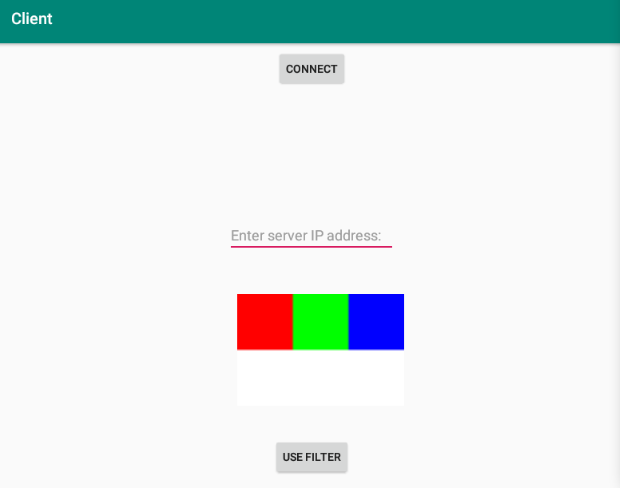
\includegraphics[width=1\textwidth]{images/client-screen.png}
    \caption{\label{fig:gui} App user interface}
\end{figure}

To apply filters, the app must preprocess the image for the device driver according to the following specification:
$32$ bit integer
ALPHA | RED |GREEN | BLUE ($8$bit|$8$bit|$8$bit|$8$bit) e.g full opaque red would be (hex notation) $FF FF 00 00$. Every pixel will be read out and saved together to a new binary file. 
The path to this file will be written to the device driver, soon after the filtered data will be read back into the UI from a new created file.

\subsubsubsection{Root client script}\label{ssssec:clientscript}
The main challenge of the Android application was the communication with the \gls{fpga} hardware in the \gls{pl}. This problem could not be solved in the previous project \cite{oldrepo}. 
In order to be able to access the FPGA hardware from the application, the app must be signed with some platform keys. However, there was no access to these keys. The installation of the app as a system app was insufficient or also required some keys.

A workaround was found. Since the application has access to the external storage, which is a specific folder on the SD card (\emph{/storage/emulated/0/SoC}), the commands to be transmitted to the kernel modules have been written to a text file.

Then a script was written that forwards the commands to the desired kernel modules called \emph{Root_Client.sh}. This script was started in the startup script and has system rights. This means that the script has access to the generated text files from the app, but also to the kernel modules.

The script is waiting for three different actions:
\begin{itemize}
    \item Control for the filter logic -- \emph{filter.txt}
    \item Control for blake2b hash function -- \emph{blake2b.txt}
    \item Control for partial reconfiguration -- \emph{partial.txt}
\end{itemize}

\textbf{Control for the filter logic:}\\
When the application performs the action to use the filter logic, a text file is created that contains the path to the bitmap file generated from the app.
The script will now check whether this text file is available or not. If the file exists, the content of the file is passed to the \emph{simple_filters} kernel module (see \cref{sssec:imageprocessingmodule}) with the \emph{echo} command. When the kernel module has finished, the result is stored in a new bitmap file.
The Android app checks whether this new bitmap file exists and continues with its further processing.
Finally, the files that are no longer needed are deleted so that no false triggering occurs.
\medbreak

\textbf{Control for blake2b hash function:}\\
When the app has downloaded a new bitstream update, the hash function need to be calculated. Therefore a text file is created that contains the path to the new bitstream file. Before the bitstream can be passed to the kernel module, the command in \cref{lst:catbitstream} must be executed. This command opens the bitstream file and sends it to a null device. If this step is not followed, the actual blake2b hash function will fail. This malfunction was only ascertained with binary files. 
\begin{lstlisting}[
	language=Bash,
	caption={Prepare bitstream for blake2b},
	label={lst:catbitstream},
	basicstyle=\small,
	float=htbp,
	floatplacement=htbp
	]
cat "$( < blake2b.txt )" > /dev/null
\end{lstlisting}

After the malfunction has been eliminated, the bitstream is passed to the \emph{blake2b} kernel module (see \cref{sssec:blake2bmodule}). The result is read from the kernel module and saved in a new text file. 
The application waits again for this file and continues its further processing. 
The files that are no longer required are deleted.
\medbreak

\textbf{Control for partial reconfiguration:}\\
If the hash from the downloaded bitstream is correct, the partial reconfiguration must be performed. The app creates a text file that contains the path to the new bitstream file. Again the commands in \cref{lst:catbitstreampr} must be executed before the partial reconfiguration can be performed. 
\begin{lstlisting}[
	language=Bash,
	caption={Prepare bitstream for partial reconfiguration},
	label={lst:catbitstreampr},
	basicstyle=\small,
	float=htbp,
	floatplacement=htbp
	]
# read path of bitstream file 
bitpath="$( < partial.txt )"
echo $bitpath > /dev/null

# read bitstream filename
bit=${bitpath##*/}
echo $bit > /dev/null
\end{lstlisting}

After the preparation, the bitstream is sent to the \gls{fpga} manager. This action is described in detail in \cref{sssec:dynamicpartialreconfiguration}.

\subsubsubsection{Server}\label{ssssec:server}
A tiny web server with a \gls{rest} API, 
written with python $3.7$ using Flask and its extension FlaskRESTful, therefore fully \gls{wsgi} compliant. However, Flask internal development server is used for the demonstration and for simplicity.

In order to use the server, the following packages available from Ubuntu repositories must be installed: 
\begin{lstlisting}[
	language=Bash,
	%caption={Install packages for the server},
	%label={lst:installserverpkg},
	basicstyle=\small,
	float=htbp,
	floatplacement=htbp
	]
sudo apt install python3 python3-pip python3-flask
pip install flask-restful 
\end{lstlisting}

Run the script at \emph{<repo>/server/run\_server.sh} to start the server. The host's IP address must be entered. The script shows all available IP addresses
Open http://<your ip>:5000 to see if the server is reachable.

There are also some preconfigured repositories implemented in a file at \emph{<repo>/server/ressources/repository.py}.
All files contained in a repository are located in the server's download folder. When a download is in progress, the server sends the file from this folder.

\subsubsubsection{Server API}\label{ssssec:serverapi}
Insomnia, a free open source \gls{rest} client available for Mac, Windows and Linux, was used for API testing and server communication (see \cref{fig:insomnia}).

\begin{figure}[htbp]
    \centering
    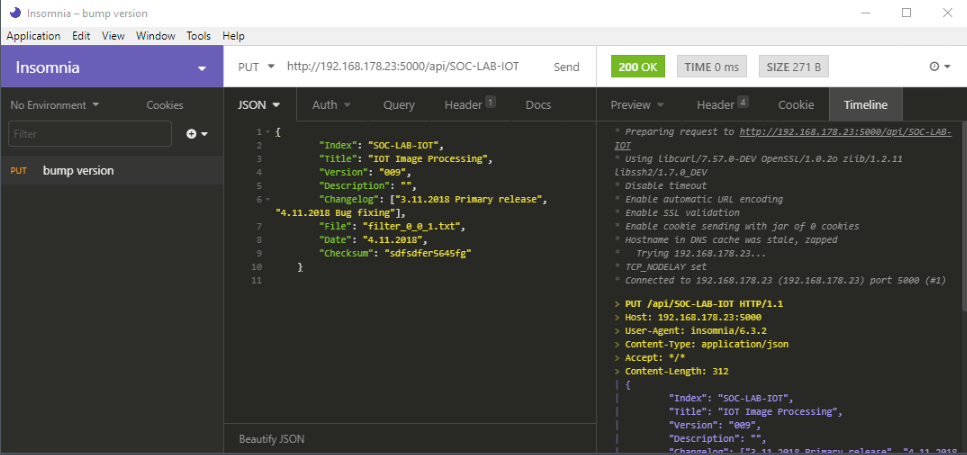
\includegraphics[width=1\textwidth]{images/insomnia.png}
    \caption{\label{fig:insomnia} Insomnia REST client}
\end{figure}

All commands of the server API are explained below.
\medbreak

\textbf{Get all information for repository <index>:}\\
This command returns all information of a requested repository. If the command is successful, the response code is $200$ otherwise it is $404$.

\begin{table}[htbp]
    \centering
    \resizebox{\textwidth}{!}{%
        \begin{tabular}{cccccc}
            \multirow{2}{*}{\textbf{URL}} & \textbf{URL} & \textbf{DATA} & \multirow{2}{*}{\textbf{METHOD}} & SUCCESS & ERROR \\
             & PARAM & PARAM &  & RESPONSE & RESPONSE \\ \hline
            /api/<index> & index=[string] & n/a & GET & 200 & 404
        \end{tabular}%
    }
\end{table}

\textbf{Create repository <index>:}\\
This command creates a new repository with the passed \gls{json} parameters. If the command is successful, the response code is $201$ otherwise it is $400$.

\begin{table}[htbp]
    \centering
    \resizebox{\textwidth}{!}{%
        \begin{tabular}{cccccc}
            \multirow{2}{*}{\textbf{URL}} & \textbf{URL} & \textbf{DATA} & \multirow{2}{*}{\textbf{METHOD}} & SUCCESS & ERROR \\
             & PARAM & PARAM &  & RESPONSE & RESPONSE \\ \hline
            /api/<index> & index=[string] & JSON & POST & 201 & 400
        \end{tabular}%
    }
\end{table}

\begin{verbatim}
JSON:
{
    "Index": "SOC-LAB-IOT",
    "Title": "IOT Image Processing",
    "Version": "001",
    "Description": "",
    "Changelog": ["3.11.2018 Primary release", "4.11.2018 Bug fixing"],
    "File": "filter_0_0_1.txt",
    "Date": "4.11.2018",
    "Checksum": ""
}	    
\end{verbatim}

\textbf{Update repository <index> or create it if not existing:}\\
This command appends the passed \gls{json} parameters to a repository or creates a new one if it does not exist. If the command changed the parameters of an existing repository, the response code is $200$, but if a new one was created, the response code is $201$.

\begin{table}[htbp]
    \centering
    \resizebox{\textwidth}{!}{%
        \begin{tabular}{cccccc}
            \multirow{2}{*}{\textbf{URL}} & \textbf{URL} & \textbf{DATA} & \multirow{2}{*}{\textbf{METHOD}} & SUCCESS & ERROR \\
             & PARAM & PARAM &  & RESPONSE & RESPONSE \\ \hline
            /api/<index> & index=[string] & JSON & PUT & 200 & 201
        \end{tabular}%
    }
\end{table}

\begin{verbatim}
JSON:
{
    "Index": "SOC-LAB-IOT",
    "Title": "IOT Image Processing",
    "Version": "002",
    "Description": "",
    "Changelog": ["3.11.2018 Primary release", 
    "4.11.2018 Bug fixing", 
    "6.11.2018 added stuff"],
    "File": "filter_0_0_4.bin",
    "Date": "6.11.2018",
    "Checksum": "fdg851dfg654dfg6541dfg65514dfghdfg45534terg"
}	
\end{verbatim}

\textbf{Delete repository <index>:}\\
This command deletes the specified repository. If the command is successful, the response code is $200$ otherwise it is $404$.

\begin{table}[htbp]
    \centering
    \resizebox{\textwidth}{!}{%
        \begin{tabular}{cccccc}
            \multirow{2}{*}{\textbf{URL}} & \textbf{URL} & \textbf{DATA} & \multirow{2}{*}{\textbf{METHOD}} & SUCCESS & ERROR \\
             & PARAM & PARAM &  & RESPONSE & RESPONSE \\ \hline
            /api/<index> & index=[string] & n/a & DELETE & 200 & 404
        \end{tabular}%
    }
\end{table}

\textbf{Download file <filename>:}\\
This command downloads the file contained in the specified repository. If the download is successful, the response code is $200$ otherwise it is $404$.

\begin{table}[htbp]
    \centering
    \resizebox{\textwidth}{!}{%
    \begin{tabular}{cccccc}
        \multirow{2}{*}{\textbf{URL}} & \textbf{URL} & \textbf{DATA} & \multirow{2}{*}{\textbf{METHOD}} & SUCCESS & ERROR \\
         & PARAM & PARAM &  & RESPONSE & RESPONSE \\ \hline
        /api/download/ & \multirow{2}{*}{filename=[string]} & \multirow{2}{*}{n/a} & \multirow{2}{*}{GET} & \multirow{2}{*}{200} & \multirow{2}{*}{404} \\
        \multicolumn{1}{l}{<path:filename>} &  &  &  &  & 
    \end{tabular}%
    }
\end{table}
